\documentclass[../ai_in_finance]{subfiles}
\usepackage[margin=1in]{geometry}
\usepackage{tikz}
\usetikzlibrary{positioning}
\usepackage{amsmath}
\usepackage{amssymb}
\usepackage{booktabs}
\usepackage{floatrow}
\usepackage{draftwatermark}

\SetWatermarkText{Wulin.Suo@Queensu.ca}
\SetWatermarkScale{0.8}
\SetWatermarkColor{gray!35}
\SetWatermarkAngle{0}
\SetWatermarkVerCenter{0.955\paperheight}

\usepackage{makeidx}
\makeindex

\begin{document}

\chapterkey{algotrading}
\chapter{Algorithmic Trading and Market Microstructure}

Every strategy considered so far in this book, from the DuPont-decomposed valuation of Chapter~\chnum{statements} to the mean-variance portfolios of Chapter~\chnum{portfolio}, has treated buying and selling an asset as instantaneous and free, so that the financial or statistical idea could be presented without execution detail. Chapter~\chnum{markets} showed this is not right: every trade costs at least half the bid-ask spread\index{bid-ask spread}, and a large enough order walks through several levels of the order book at a progressively worse price. This chapter treats execution as a subject in its own right: how a trading signal is generated, how an order is worked in the market, how a strategy's historical performance should be evaluated, and how market microstructure shapes each of those decisions.\index{market microstructure}

Several worked examples run through the chapter, each grounded in earlier material. A moving-average crossover strategy, backtested on a short synthetic price series, shows how a signal becomes a sequence of positions and then a profit-and-loss series. The limit-order-book walk from Chapter~\chnum{markets} is extended into a comparison of aggressive, single-shot execution with a patient, multi-slice alternative, motivating the TWAP\index{TWAP (time-weighted average price)} and VWAP\index{VWAP (volume-weighted average price)} benchmarks, and into a regression estimate of Kyle's lambda\index{Kyle model} that gives price impact an economic interpretation.

The market-making intuition of Chapter~\chnum{markets} is developed into a worked Avellaneda-Stoikov\index{Avellaneda-Stoikov model} inventory example, showing how and why a market maker's quotes should skew as its position grows.

The pairs-trading setup of Chapter~\chnum{timeseries} becomes a backtested trade, entered and exited with the $z$-score rule that chapter only described, and is then generalized into a multi-stock statistical arbitrage example built on Chapter~\chnum{portfolio}'s factor regressions.

Chapters~\chnum{ml} and~\chnum{timeseries} supplied the tools to generate a trading signal; Chapter~\chnum{portfolio} supplied the logic for combining assets and signals into a position. This chapter supplies the missing link: everything that happens after a model or optimizer has decided what to hold, and before that decision becomes a completed trade at a real, imperfect price. Treating execution as instantaneous and free is the simplifying assumption every earlier chapter made for clarity; this chapter shows what it costs when it is relaxed.

\section{Trading Signals and a First Strategy}

Every algorithmic strategy begins with a signal, a rule that turns observable data into a view about where a price is going. This part classifies the signals the industry trades and works one of the simplest through, from raw prices to a realized return.

\subsection{A Taxonomy of Trading Strategies and Signals}
\label{sec:taxonomy}\index{algorithmic trading!taxonomy of strategies}

Suppose two traders notice the same pattern in a stock's recent price history but reach opposite conclusions: one buys, betting a recent rise will continue; the other sells short, betting the rise has gone too far and must reverse. Both can be running a coherent strategy; they disagree about the economic source of the pattern.

Strategies are usually organized by that source. Momentum strategies bet that a recent price trend will continue\index{momentum}\index{trading signal!momentum}, on the theory that information diffuses gradually through a market rather than being reflected in prices instantly. Mean-reversion strategies bet the opposite\index{mean reversion}\index{trading signal!mean reversion}: that a price, or a relationship between two prices as in this chapter's pairs trade, has moved too far from a fundamental or statistical anchor and will revert, an application of Chapter~\chnum{timeseries}'s stationarity concepts. Market-making strategies (Section~\ref{sec:inventory}) take no directional view\index{market making}, profiting from repeatedly capturing the bid-ask spread while managing the resulting inventory risk. Statistical arbitrage generalizes mean reversion to many assets\index{statistical arbitrage}, often using Chapter~\chnum{portfolio}'s factor models to find a stable relationship.

Each strategy type produces the same output: a signal\index{trading signal}, a number (or a direction) indicating whether and how much to buy or sell at a given time. Converting that signal into a position, and the position into executed trades, is the concern of most of this chapter, a step with its own economics, costs, and risks, separate from whether the signal is any good.

\weheading{\subsection}{algotrading-ma-crossover}{A Moving-Average Crossover Strategy}\index{moving-average crossover strategy}
\label{sec:ma-crossover}

A moving-average crossover strategy, one of the oldest and most transparent momentum strategies, holds a long position whenever a short-window moving average is above a longer-window one\index{moving average!simple}\index{trend following}, and is flat otherwise, on the theory that the crossing signals a strengthening upward trend. Table~\ref{tab:ma_crossover} applies a 3-day short average and a 6-day long average to twelve days of hypothetical prices.

\begin{booktable}[htbp]{A 3-day/6-day moving-average crossover strategy}{tab:ma_crossover}
\begin{tabular}{lrrrrr}
\toprule
Day & Price & MA(3) & MA(6) & Signal & Strategy Return \\
\midrule
1  & 100 & --     & --     & 0 & -- \\
2  & 101 & --     & --     & 0 & 0.00\% \\
3  & 103 & 101.33 & --     & 0 & 0.00\% \\
4  & 106 & 103.33 & --     & 0 & 0.00\% \\
5  & 110 & 106.33 & --     & 0 & 0.00\% \\
6  & 115 & 110.33 & 105.83 & 1 & 0.00\% \\
7  & 119 & 114.67 & 109.00 & 1 & 3.48\% \\
8  & 118 & 117.33 & 111.83 & 1 & $-0.84\%$ \\
9  & 114 & 117.00 & 113.67 & 1 & $-3.39\%$ \\
10 & 109 & 113.67 & 114.17 & 0 & $-4.39\%$ \\
11 & 104 & 109.00 & 113.17 & 0 & 0.00\% \\
12 & 100 & 104.33 & 110.67 & 0 & 0.00\% \\
\bottomrule
\end{tabular}
\end{booktable}

The signal turns on (long) at day 6, when the 3-day average first exceeds the 6-day average, and turns off (flat) at day 10, when it first falls back below. Crucially, the strategy return in each row applies the \emph{previous} day's signal to the \emph{current} day's price return. A signal computed from today's close cannot be traded until the next available price, the point-in-time discipline Chapter~\chnum{ml} emphasized against data leakage\index{data leakage!look-ahead}; using today's signal against today's return would silently look ahead.

Compounding the strategy returns gives a cumulative return of $-5.22\%$ over the twelve days, while buying and holding from day 1 to day 12 (starting and ending at 100) returns $0\%$. In this sample the crossover strategy underperforms buy-and-hold: it captures part of the days-6-through-8 uptrend but stays long one day too long into the days-9-and-10 reversal, the whipsaw risk that afflicts every momentum strategy\index{trend following!whipsaw} at a trend reversal. The example is deliberately not a success story: a backtest evaluation (Section~\ref{sec:backtest-metrics}) must be prepared to find that a plausible strategy does not work on the available data.

\section{Execution and Market Impact}

A signal is only half a strategy. Turning a desired position into an actual one means sending orders into a market that moves in response, so this part develops the mechanics of execution, the cost of demanding liquidity too quickly, and the models that balance that cost against the risk of trading too slowly.

\subsection{Order Types and the Mechanics of Execution}\index{order types}

Chapter~\chnum{markets} introduced the market order (executed immediately\index{order types!market order} at the best available price, walking through the book if necessary) and the limit order (executed only\index{order types!limit order} at a specified price or better, potentially never filling at all). Converting a signal like the one in Section~\ref{sec:ma-crossover} into a position requires choosing among these order types, a direct trade-off: a market order guarantees execution but accepts whatever price impact results, while a limit order controls the price but risks never filling if the market moves away before the order reaches the front of the queue. A stop order\index{order types!stop order} becomes a market order once a trigger price is reached, commonly used to implement a predetermined exit rule (a stop-loss)\index{stop-loss} without continuous monitoring.

An execution system must also decide how to route an order, since modern equity markets consist of many competing exchanges and alternative venues rather than one centralized book, a fragmentation Chapter~\chnum{markets} touched on\index{market fragmentation} in its discussion of Regulation NMS\index{Regulation NMS (Reg NMS)}. A smart order router evaluates liquidity and price across every venue and splits or directs an order to capture the best aggregate execution, a harder problem than the single-book walk but built on the same economics of price and available size at each level.

A large order also raises a tension the order types above do not resolve: posting the full order as a visible limit order reveals the trader's intentions to other participants, who can respond, for example by front-running the anticipated remaining demand. Iceberg orders\index{iceberg orders}\index{order types!iceberg order} address this by displaying only a small portion of the order at a time, revealing more as the visible portion fills. Dark pools\index{dark pools} go further: private venues that match buy and sell orders without displaying any pre-trade price or size, reporting only completed trades after the fact.

Both mechanisms trade away pre-trade transparency, one of the market-quality benefits Chapter~\chnum{markets} attributed to well-functioning exchanges, for reduced information leakage and, in principle, lower market impact\index{market impact} for large orders. It is a trade-off, not a free improvement: when a large fraction of volume trades in non-displayed venues, the lit order book becomes a less complete picture of supply and demand, a concern regulators have studied as dark-pool volume has grown. In 2025, for the first time, more than half of U.S. equity volume executed off-exchange, most of it not in dark pools but through wholesale market makers that pay retail brokers for their order flow and internalize it\index{payment for order flow}\index{internalization}. Chapter~\chnum{hft}'s section on U.S. equity market structure as of 2026 dates that figure and the rule changes that followed it, among them a half-penny tick, lower access-fee caps, new round-lot sizes, and expanded execution-quality reports under Rule 605, all of which change the inputs a smart order router works with.

Figure~\ref{fig:execution_pipeline} places these decisions in sequence. A signal is generated, an order type is chosen, a venue is selected, and the resulting execution is measured, with that measurement feeding back into how the next signal is traded. The rest of this chapter works through that loop one stage at a time; every stage introduces costs the signal never sees.

\begin{bookfigure}[htbp][The path from a trading signal to a completed, evaluated trade]{The path from a trading signal to a completed, evaluated trade: each stage introduces its own decisions and costs, and transaction cost analysis at the end feeds back into how future signals and execution choices are made}{fig:execution_pipeline}
    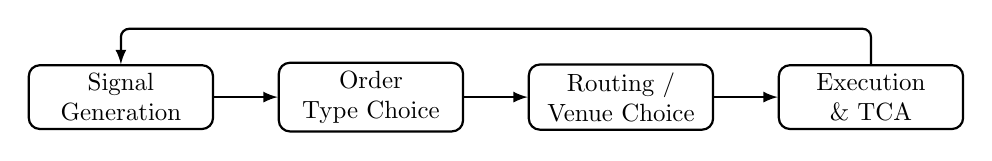
\begin{tikzpicture}[>=latex,thick,node distance=0.9cm,scale=0.9,transform shape]
        \node[draw,rounded corners,minimum width=2.6cm,minimum height=0.9cm,align=center] (signal) {Signal\\Generation};
        \node[draw,rounded corners,minimum width=2.6cm,minimum height=0.9cm,right=of signal,align=center] (order) {Order\\Type Choice};
        \node[draw,rounded corners,minimum width=2.6cm,minimum height=0.9cm,right=of order,align=center] (route) {Routing /\\Venue Choice};
        \node[draw,rounded corners,minimum width=2.6cm,minimum height=0.9cm,right=of route,align=center] (exec) {Execution\\\& TCA};
        \draw[->] (signal) -- (order);
        \draw[->] (order) -- (route);
        \draw[->] (route) -- (exec);
        % Orthogonal feedback route rather than a bezier arc: a to[out=135,in=45]
        % curve bulges in proportion to the chain's width, and across four boxes it
        % claimed more vertical space than the boxes themselves. This rises a fixed
        % 0.5cm whatever the chain's width. Same fix as Chapter 6's lifecycle figure.
        \draw[->,rounded corners=3pt] (exec.north) -- ++(0,0.5) -| (signal.north);
    \end{tikzpicture}
\end{bookfigure}

\subsection{Market Impact and the Cost of Trading Fast}
\label{sec:market-impact}

Chapter~\chnum{markets}'s limit-order-book example showed that a 250-share market order, larger than the 100 shares available at the best ask of \$50.10, walked through a second price level and executed at an average price of \$50.13\index{limit order book!walking the book}, a price impact of about 6 basis points relative to the best ask. This cost arises entirely from the order's size relative to available liquidity; it is not a fee but the consequence of consuming the supply at each successive price level.

The alternative is to break the order into smaller pieces spaced over time, letting the book replenish between slices. Suppose the 250-share order is split into five 50-share slices, each small enough to fill within the 100 shares at the best ask, and suppose the best ask stays at \$50.10 between slices (a simplification; in reality the book may not fully replenish, and the price may drift for reasons unrelated to this trader).

This patient approach achieves an average price of \$50.10, eliminating the price impact, but at a cost the single-shot execution does not bear: while five slices are worked, the price can move for unrelated reasons, a risk called timing risk or execution risk\index{timing risk}\index{optimal execution!timing risk}. The aggressive strategy pays a known impact cost immediately; the patient one pays an expected impact cost of zero but accepts an uncertain timing-risk cost. Neither is universally superior; the choice depends on order size relative to liquidity, the asset's volatility, and urgency, the trade-off formalized in Section~\ref{sec:optimal-execution}.

\subsection{The Kyle Model: A Formal Model of Price Impact}
\label{sec:kyle-model}

The order-book walk demonstrates price impact mechanically but does not explain \emph{why} a market maker sets prices that respond to order flow. The classic model of \textcite{kyle1985continuous} supplies the explanation: a market maker cannot distinguish an informed trader\index{informed trading} (who knows something about the asset's true value) from a liquidity trader (who trades for unrelated reasons, such as needing cash), and must set a single price schedule that breaks even on average against this mixture. Its rational response is to move the price in proportion to the net signed order flow it observes,\index{order flow}
\begin{equation}
\Delta P = \lambda \times (\text{Net Order Flow}) + \varepsilon,
\label{eq:algotrading-kyle}
\end{equation}
where net order flow is buy volume minus sell volume over some interval and $\lambda$ (Kyle's lambda) measures the price impact per unit of net order flow\index{Kyle's lambda}\index{market impact!Kyle's lambda}, estimated by regressing observed price changes on net order flow.

Table~\ref{tab:kyle_data} shows six intervals of net order flow (in thousands of shares) and the resulting price change (in cents).

\begin{booktable}[htbp]{Net order flow and price change for estimating Kyle's lambda}{tab:kyle_data}
\begin{tabular}{lrrrrrr}
\toprule
Interval & 1 & 2 & 3 & 4 & 5 & 6 \\
Net order flow (000s) & 5 & $-3$ & 8 & $-6$ & 2 & 4 \\
Price change (cents) & 10 & $-7$ & 15 & $-11$ & 3 & 9 \\
\bottomrule
\end{tabular}
\end{booktable}

Applying the same OLS formula used since Chapter~\chnum{ml},
\begin{equation*}
\hat\lambda = \frac{\sum_t (\text{Flow}_t - \overline{\text{Flow}})(\Delta P_t - \overline{\Delta P})}{\sum_t (\text{Flow}_t-\overline{\text{Flow}})^2} \approx 1.95 \text{ cents per thousand shares}, \qquad R^2 \approx 0.99.
\end{equation*}
A larger $\lambda$ means prices move more sharply for a given net buying or selling pressure, which Kyle's model interprets as informed trading being a larger fraction of order flow, or liquidity (the order-book depth available to absorb flow) being thinner. This gives price impact an economic interpretation: it is compensation the market maker requires for the risk of unknowingly trading against better-informed counterparties, the adverse-selection component of the spread\index{bid-ask spread!adverse-selection component}\index{adverse selection!in market making} introduced in Chapter~\chnum{markets}, now a single estimable slope.

One caution, because everything built on that slope inherits it: $\hat\lambda$ is estimated as a constant, and it is not one. Impact per unit of order flow varies with the time of day, widest around the open and narrowest in the quiet afternoon; with the volatility regime; and with order size, since a larger order walks into thinner depth. A production pre-trade cost model therefore fits a conditional impact surface\index{market impact}, regressing realized impact on order size, participation rate, quoted spread, volatility, and time of day, Chapter~\chnum{ml}'s supervised-learning setup pointed at execution. Kyle's constant $\lambda$ makes the economics legible; the fitted surface is what a desk budgets against.

\subsection{TWAP and VWAP: Basic Execution Algorithms}
\label{sec:twap-vwap}\index{execution algorithms!TWAP}\index{execution algorithms!VWAP}

The multi-slice approach in Section~\ref{sec:market-impact} is a simple version of the time-weighted average price (TWAP) algorithm: split an order into equal slices spread evenly across a horizon, without reference to how volume is distributed over it. Table~\ref{tab:twap_vwap} shows five hypothetical intervals with market prices and total trading volume.

\begin{booktable}[htbp]{Prices and market volume over five execution intervals}{tab:twap_vwap}
\begin{tabular}{lrrrrr}
\toprule
Interval & 1 & 2 & 3 & 4 & 5 \\
Price & \$50.00 & \$50.05 & \$50.10 & \$50.08 & \$50.12 \\
Market volume & 10{,}000 & 12{,}000 & 8{,}000 & 15{,}000 & 9{,}000 \\
\bottomrule
\end{tabular}
\end{booktable}

A trader executing a 1,000-share order via TWAP trades 200 shares in each interval regardless of volume, achieving an average execution price equal to the simple average of the five prices,
\begin{equation*}
\text{TWAP execution price} = \frac{50.00+50.05+50.10+50.08+50.12}{5} = \$50.07.
\end{equation*}
The volume-weighted average price (VWAP) benchmark, by contrast, weights each interval's price by that interval's share of total market volume,
\begin{equation*}
\text{VWAP} = \frac{\sum_t P_t V_t}{\sum_t V_t} = \frac{50.00(10{,}000)+\cdots+50.12(9{,}000)}{10{,}000+12{,}000+8{,}000+15{,}000+9{,}000} \approx \$50.068,
\end{equation*}
close to the TWAP execution price, a difference of about 0.4 basis points. The gap turns on which intervals carried the volume: the two most expensive intervals, the third at \$50.10 and the fifth at \$50.12, drew the least volume, $8{,}000$ and $9{,}000$ shares, so volume weighting puts the least weight where the price was worst for a buyer. Interval 4 carries the largest volume, $15{,}000$ shares, but at \$50.08 it sits a cent \emph{above} the TWAP average and nudges the weighted price the other way. A VWAP-following algorithm would have traded proportionally less in the two expensive intervals than TWAP did, capturing a slightly better average price. In practice, a VWAP algorithm trades according to a historical intraday volume profile, since the day's volume is not known in advance. The theory is that trading when the market is naturally most liquid minimizes the trader's footprint and price impact.

That contains a forecasting problem, and it is the hard part of the algorithm. Trading to VWAP requires knowing how the day's volume will be distributed before the day is over, and a historical average profile is the crudest forecast of it. Volume departs from that profile for partly predictable reasons: an index rebalance, an earnings release, an options expiry, or a heavy opening auction all bend the curve in ways a static profile cannot anticipate. Predicting the intraday volume curve is a supervised regression problem in Chapter~\chnum{timeseries}'s sense, with the day's realized volume so far as the most informative feature, and it demands the same walk-forward evaluation.\index{walk-forward validation} An execution desk treats this forecast, not the weighting formula, as where a VWAP algorithm is won or lost.

\subsection{Optimal Execution: Balancing Impact and Timing Risk}
\label{sec:optimal-execution}\index{optimal execution}

Section~\ref{sec:market-impact}'s comparison of aggressive and patient execution is a simplified version of the optimal execution problem formalized by Almgren and Chriss\index{Almgren-Chriss model}. Given an order of fixed size that must be completed by a fixed deadline, how should it be split over time to minimize expected market impact cost plus the variance introduced by timing risk? Impact cost is typically modeled as increasing in the trading rate, since trading faster consumes more of the liquidity at each price level, as in Chapter~\chnum{markets}'s order-book walk. Timing risk increases with the time the order remains unexecuted, since a longer horizon exposes the remaining quantity to more adverse price movement, the variance-grows-with-horizon logic of Chapter~\chnum{timeseries}'s multi-step forecasts.

The framework's output is not a single number but an efficient frontier\index{efficient frontier} analogous to Chapter~\chnum{portfolio}'s risk-return frontier. For each level of acceptable timing risk there is an optimal trajectory that minimizes expected cost, typically front-loaded, trading more aggressively early and tapering off. A more risk-averse trader, who weights the variance of the outcome more heavily, will choose a faster, more front-loaded execution than a less risk-averse trader facing the same order and market.

This formalizes the trade-off Section~\ref{sec:market-impact} described qualitatively: neither extreme is generally optimal, and the answer depends on impact sensitivity and price volatility, which must be estimated from data, with all the estimation-error caveats Chapter~\chnum{portfolio} raised.

\weheading{\subsection}{algotrading-almgren-chriss}{The Almgren-Chriss Optimal Trajectory}\index{Almgren-Chriss model}

Almgren and Chriss formalize the trade-off above by minimizing a risk-adjusted total cost, expected temporary-impact cost plus $\phi$ times its variance from timing risk, where $\phi\ge 0$ is the trader's risk-aversion parameter (written $\phi$ here rather than the $\lambda$ of Almgren and Chriss's own paper, to keep it distinct from Kyle's lambda above),
\begin{equation}
\min_{x_1,\ldots,x_{N-1}} \; \underbrace{\eta\sum_{j=1}^N \frac{(x_{j-1}-x_j)^2}{\tau}}_{\text{expected impact cost}} \; + \; \phi\underbrace{\sigma^2\tau\sum_{j=1}^N x_j^2}_{\text{timing-risk variance}},
\label{eq:algotrading-ac-objective}
\end{equation}
where $x_j$ is the number of shares still unexecuted after interval $j$ (so $x_0=X$, the full order, and $x_N=0$, fully executed), $\tau$ is the length of each interval, $\eta$ is the temporary-impact cost coefficient, and $\sigma$ is the volatility of the share \emph{price}, in dollars per share per unit of time, so that $\sigma^2\tau$ is the variance of the price change over one interval. The units matter: $\sigma$ multiplies share counts in the variance term, so it must be a price volatility, not a percentage return volatility. The closed-form solution to this minimization is\index{Almgren-Chriss model!optimal trajectory}\index{optimal execution!Almgren-Chriss}
\begin{equation}
x_j = X\,\frac{\sinh(\kappa(T-t_j))}{\sinh(\kappa T)}, \qquad \kappa=\sqrt{\frac{\phi\sigma^2}{\eta}},
\label{eq:algotrading-ac-trajectory}
\end{equation}
with $T=N\tau$ the total horizon; $\kappa$ governs how front-loaded the trajectory is, growing with risk aversion $\phi$ and volatility $\sigma$ and shrinking with impact cost $\eta$. The trajectory is stated without proof; the companion technical note on the Almgren-Chriss model derives it from the discrete first-order condition, a linear second-order difference equation, and verifies the two limiting cases: uniform, TWAP-style trading as risk aversion vanishes, and immediate liquidation as it grows without bound.

Applying this to Section~\ref{sec:market-impact}'s $250$-share order split across the same $N=5$ intervals, with each interval taken as the unit of time ($\tau=1$) and illustrative parameters $\sigma=\$0.02$ per share per interval, $\eta=0.01$, and a modest risk aversion of $\phi=0.5$ (so $\kappa\approx0.1414$), the optimal trajectory leaves
\begin{align*}
\text{Unexecuted shares:} &\quad x=(250,\ 194.2,\ 142.4,\ 93.4,\ 46.2,\ 0), \\
\text{Traded per interval:} &\quad (55.8,\ 51.9,\ 49.0,\ 47.1,\ 46.2),
\end{align*}
mildly front-loaded relative to the perfectly uniform $50$-share-per-interval TWAP schedule of Section~\ref{sec:market-impact}. Raising risk aversion tenfold to $\phi=5$ (so $\kappa\approx0.4472$) sharpens this front-loading considerably,
\begin{align*}
\text{Traded per interval:} &\quad (92.8,\ 60.9,\ 41.3,\ 30.1,\ 25.0),
\end{align*}
nearly double the first-interval quantity of the low-risk-aversion trajectory: a more risk-averse trader accepts a higher expected impact cost up front to shrink the variance from the part of the order still exposed to price moves. Figure~\ref{fig:almgren_chriss_trajectories} plots both trajectories against the uniform TWAP baseline, showing how the front-loading grows with $\phi$.

\begin{bookfigure}[htbp]{Almgren-Chriss optimal unexecuted-share trajectories at two risk-aversion levels, against the uniform TWAP baseline}{fig:almgren_chriss_trajectories}
    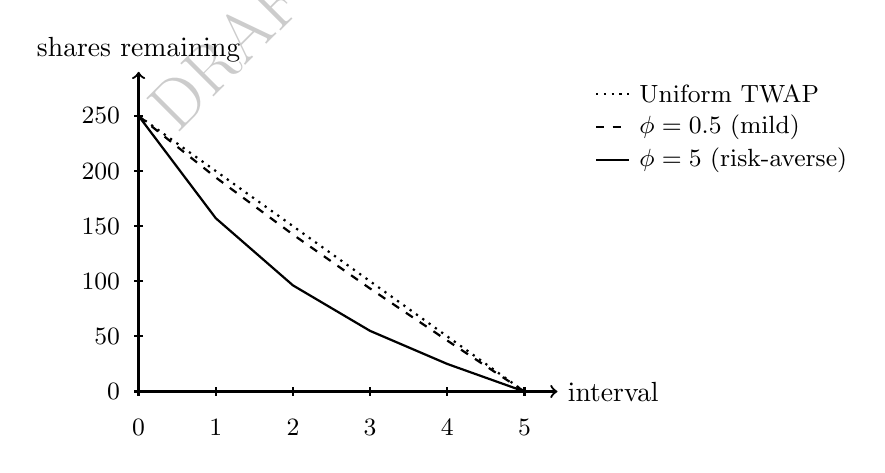
\begin{tikzpicture}[thick,scale=0.7]
        \draw[->] (0,0) -- (7.6,0) node[right] {interval};
        \draw[->] (0,0) -- (0,5.8) node[above] {shares remaining};
        \foreach \i in {0,1,2,3,4,5} {
            \draw (\i*1.4,0.08) -- (\i*1.4,-0.08);
            \node[below,font=\small] at (\i*1.4,-0.32) {\i};
        }
        \foreach \y/\lab in {0/0,1/50,2/100,3/150,4/200,5/250} {
            \draw (0.08,\y) -- (-0.08,\y);
            \node[left,font=\small] at (-0.15,\y) {\lab};
        }
        \draw[dotted] plot coordinates {(0,5) (1.4,4) (2.8,3) (4.2,2) (5.6,1) (7.0,0)};
        \draw[dashed] plot coordinates {(0,5) (1.4,3.884) (2.8,2.848) (4.2,1.868) (5.6,0.924) (7.0,0)};
        \draw[solid] plot coordinates {(0,5) (1.4,3.144) (2.8,1.926) (4.2,1.10) (5.6,0.5) (7.0,0)};
        \draw[dotted] (8.3,5.4) -- (8.9,5.4); \node[right,font=\small] at (8.9,5.4) {Uniform TWAP};
        \draw[dashed] (8.3,4.8) -- (8.9,4.8); \node[right,font=\small] at (8.9,4.8) {$\phi=0.5$ (mild)};
        \draw[solid] (8.3,4.2) -- (8.9,4.2); \node[right,font=\small] at (8.9,4.2) {$\phi=5$ (risk-averse)};
    \end{tikzpicture}
\end{bookfigure}

Scoring the optimal trajectory, the uniform TWAP schedule, and the single-shot execution of Section~\ref{sec:market-impact} on the same risk-adjusted objective at $\phi=0.5$ makes the trade-off concrete:
\begin{align*}
\text{Optimal trajectory:} &\quad \text{cost} = 139.4, \\
\text{Uniform TWAP:} &\quad \text{cost} = 140.0, \\
\text{Fully aggressive single-shot:} &\quad \text{cost} = 625.0,
\end{align*}
the TWAP schedule barely worse since $\phi=0.5$ is only mildly risk-averse, and the single-shot execution over four times worse, since it eliminates timing risk but pays a quadratically larger impact cost for trading the whole order in one interval. Both extremes are feasible points, but neither is optimal once risk aversion is weighed against expected cost, and the front-loaded shape of the optimum is not a generic property of ``spreading an order out'' but the output of this closed-form solution.

The costs above are in dollars, with $\phi$ measured per dollar, and the units are a common source of error. On the \$50 stock of the order-book example, $\sigma=\$0.02$ per share per interval is a return volatility of $0.04\%$ per interval; with five intervals to the trading day it scales by the square-root-of-time rule\index{square-root-of-time rule} to $0.0894\%$ a day and $1.42\%$ a year, a deliberately calm stock chosen to keep the numbers readable. Going the other way, a typical $25\%$ annual volatility on the same stock converts to $0.25\times\$50/\sqrt{252\times5}=\$0.3521$ per share per interval. The mistake the units guard against is entering a percentage directly: reading $\sigma=0.02$ as a $2\%$ return volatility on a \$50 stock means $\sigma=\$1.00$, which makes $\kappa=7.07$, fifty times larger, and an optimal schedule that sells $249.8$ of the $250$ shares in the first interval.

The objective in Equation~\eqref{eq:algotrading-ac-objective} also contains only the \emph{temporary} impact of each slice, the premium paid to consume liquidity, which leaves the price for later slices untouched. Almgren and Chriss also model a \emph{permanent} impact\index{market impact!permanent}\index{market impact!temporary}: every share sold lowers the price for all later shares by $\gamma$, because the market reads the order flow as information. With linear permanent impact its expected cost is $\gamma X^2/2$ minus a small term, $\tfrac{\gamma}{2}\sum_j(x_{j-1}-x_j)^2$, that depends on the schedule in the same way as the temporary cost and so lowers the effective temporary coefficient from $\eta/\tau$ to $\eta/\tau-\gamma/2$. At an illustrative $\gamma=\$0.002$ per share per share sold, the permanent cost is $\$62.50-\$12.56=\$49.94$ for the optimal trajectory and $\$62.50-\$12.50=\$50.00$ for TWAP: a substantial cost, but almost the same for every gradual schedule, which is why the optimal trajectory is usually stated with temporary impact alone. Permanent impact matters a great deal for \emph{how much} to trade, as the next section shows, and hardly at all for \emph{how to spread} a given order.

The closed form's assumptions are stronger than its elegance suggests. The trajectory is optimal only if impact is linear in the trading rate, volatility is constant across the horizon, and the trader has no view on where the price is heading. All three are false in ways any execution desk would recognize, and relaxing any one destroys the closed form. What survives is the problem: choosing a sequence of trade sizes to minimize expected cost plus a risk penalty is a sequential decision problem, solvable by learning a policy from simulated episodes\index{optimal execution!reinforcement learning} instead of solving a difference equation. Chapter~\chnum{rl} does this, recovering the trajectory above for the same parameters with tabular Q-learning, then extending it to frictions the closed form cannot express.

\subsection{The Square-Root Law and Strategy Capacity}
\label{sec:square-root-impact}\index{market impact!square-root law}

Kyle's model and the Almgren-Chriss objective both treat impact as linear in the amount traded, a reasonable local approximation for a single small slice. For a whole \emph{metaorder}, the full parent order a fund works over hours or days, the best-documented empirical regularity in market microstructure says otherwise. Across stocks, markets, and decades, the average price impact of a metaorder of $Q$ shares grows with the square root of its size,
\begin{equation}
\frac{\Delta P}{P} \approx Y\,\sigma_{\text{daily}}\sqrt{\frac{Q}{V}},
\label{eq:algotrading-square-root}
\end{equation}
where $V$ is the stock's average daily volume, $\sigma_{\text{daily}}$ its daily return volatility, and $Y$ a constant of order one \parencite{toth2011anomalous}. Studies of large institutional order sets find the same concave shape, with fitted exponents close to one half; \textcite{almgren2005direct}, on Citigroup's U.S. equity orders, preferred a slightly steeper $3/5$. Two features make the law useful. Volatility and daily volume, both easy to measure, carry most of the cross-sectional variation in impact. And concavity changes the arithmetic of size: with $Y=1$ and $2\%$ daily volatility, an order for $1\%$ of daily volume costs about $0.02\times\sqrt{0.01}=20$ basis points, and one for $4\%$ costs $40$. Quadrupling the order doubles the cost per share, so the total dollar cost rises eightfold, as $Q^{3/2}$.

The square-root law describes the \emph{peak} impact at the end of a metaorder, which is largely temporary: once buying stops, a substantial part of the price move reverts over the following hours, and the part that remains is the permanent, information-driven component of the previous section \parencite{bacry2015market}. The distinction is economically sharp. A fund pays the peak on every share it trades but keeps only the permanent part as a mark-to-market gain on the position it built.

The law's most important application is the question every strategy eventually faces: how much capital can it run? Consider a strategy that rebalances monthly into 50 stocks, each trading \$50 million a day, turning over its whole book at each rebalance. Every trade carries a gross expected alpha of $50$ basis points of the value traded and pays a $3$ basis point half-spread plus square-root impact with $Y=1$ and $2\%$ daily volatility. With assets under management $A$, each stock receives a trade of $A/50$, so the net alpha per trade is
\begin{equation*}
\alpha_{\text{net}}(A) = 50 - 3 - 200\sqrt{\frac{A/50}{\$50\text{ million}}} \quad\text{basis points}.
\end{equation*}
At \$10 million the trades are $0.4\%$ of daily volume and net alpha is $34.35$ basis points; at \$100 million they are $4\%$ of volume and only $7.00$ basis points survive; net alpha reaches zero at \$138.1 million, and at \$200 million each rebalance loses money. The capacity that matters to the manager is not that break-even point but the size that maximizes total dollar profit, $A\,\alpha_{\text{net}}(A)$. Because impact grows as $\sqrt{A}$, profit $A(a - k\sqrt{A})$ is maximized where $k\sqrt{A}=2a/3$, which leaves exactly one third of the pre-impact edge $a$ as net alpha. Here that is \$61.4 million, with $15.67$ basis points of net alpha per trade and about \$96,000 of profit per rebalance, \$1.15 million a year. Growing the fund to \$100 million would cut its profit per rebalance to \$70,000, though still well short of break-even. Gross alpha that looks robust in a backtest at small size can support only a modest fund, and the square-root law puts a number on it, which a linear-impact model, with its constant cost per share, cannot do.

\section{Inventory Models and Market Making}
\label{sec:inventory}\index{inventory models}\index{market making!inventory models}

Chapter~\chnum{markets} introduced market making: a market maker profits from the bid-ask spread by standing ready to buy and sell, but bears inventory risk\index{inventory risk}\index{market maker!inventory risk} from holding a nonzero position while waiting for an offsetting order. The Avellaneda-Stoikov model formalizes this by having the market maker adjust both quotes based on current inventory, not just on fair value. A market maker with a large long position, from selling less than buying, should skew both quotes downward: a lower bid makes it less attractive for others to sell to it, and a lower ask makes it more attractive to buy from it. That works the inventory back toward zero rather than waiting for random order flow to do so.

The model formalizes this skew through a reservation price\index{Avellaneda-Stoikov model!reservation price}, the price at which the market maker would be indifferent to a marginal trade given its inventory, which sits below the mid price when it is long and above it when short,
\begin{equation}
r = s - q\,\gamma\,\sigma^2\,(T-t),
\label{eq:algotrading-as-reservation}
\end{equation}
where $s$ is the current mid price, $q$ is the current inventory (positive if long, negative if short), $\gamma$ is a risk-aversion parameter, $\sigma^2$ is the asset's return variance, and $T-t$ is the time remaining in the trading horizon. The optimal bid and ask are centered on this reservation price, not on the mid price, and separated by an optimal spread\index{Avellaneda-Stoikov model!optimal spread}
\begin{equation}
\delta = \gamma\sigma^2(T-t) + \frac{2}{\gamma}\ln\left(1+\frac{\gamma}{\kappa}\right),
\label{eq:algotrading-as-spread}
\end{equation}
where $\kappa$ governs how sensitively order arrival rates respond to how competitively the market maker quotes. Consider a market maker with mid price $s=\$100$, long $q=5$ units, $\gamma=0.1$, $\sigma=2$, one unit of time remaining ($T-t=1$), and $\kappa=1.5$. The reservation price is $r = 100 - 5(0.1)(2^2)(1) = \$98.00$, two dollars below the mid price, reflecting the desire to reduce the long position. Both formulas are quoted rather than derived; the companion technical note on the Avellaneda-Stoikov model derives the reservation price from exponential (CARA) utility applied to a normally distributed terminal mark-to-market value, and the per-side markup from the Poisson arrival intensity, which is why the spread decomposes into an inventory-risk term that vanishes as the horizon closes and an order-arrival term that does not. The optimal spread works out to $\delta \approx \$1.69$, giving
\begin{align*}
\text{Inventory-aware quotes:} &\quad \text{bid} = r-\delta/2\approx\$97.15, \ \text{ask} = r+\delta/2\approx\$98.85, \\
\text{Naive quotes (ignoring inventory):} &\quad \text{bid} = \$99.15, \ \text{ask} = \$100.85,
\end{align*}
the inventory-aware quotes both \$2.00 lower, the reservation-price adjustment carried through to each side. The ask becomes more attractive to a buyer (encouraging trades that reduce the long position) and the bid less attractive to a seller (discouraging trades that would increase it), while the $\$1.69$ spread, and so the expected compensation per round trip, is unchanged.

This skewing connects to the spread decomposition of Chapter~\chnum{markets}: the inventory-holding component of the spread\index{bid-ask spread!inventory component} is the compensation a market maker requires for the risk that its inventory moves against it before an offsetting trade arrives, and Avellaneda-Stoikov derives the optimal quote adjustment as a function of inventory, remaining horizon, and volatility. The skew grows with $\gamma$, $\sigma^2$, and the position $q$: a more risk-averse market maker, a more volatile asset, or a larger position all call for a more aggressive skew, since inventory risk is more urgent to offload when it is larger or more dangerous to hold. A market maker who quotes a fixed spread around fair value regardless of position is exposed to accumulating, unhedged directional risk, an instance of the risk management discipline of Chapter~\chnum{marketrisk}.

The caveat of Section~\ref{sec:optimal-execution} applies here too, for the same reason. Avellaneda-Stoikov is solvable in closed form because order arrivals are Poisson with fixed intensity, volatility is constant, and the only state that matters is inventory and time remaining. A market maker in a real book faces arrivals that cluster, counterparties whose order flow carries information the model's symmetric arrivals cannot represent, and a choice of venue on top of the choice of quote. Learned quoting policies exist to handle these\index{market making!reinforcement learning for}, which is why Chapter~\chnum{rl} rebuilds this model as a reinforcement learning problem. The closed form is still the right thing to meet first: it explains \emph{why} quotes should skew toward inventory and by how much, a question no learned policy will answer for you.

\section{Arbitrage and Relative-Value Strategies}\index{relative-value strategies}\index{arbitrage}

Momentum and market making both take a view on a single instrument. A third family instead trades the relationship between instruments, holding offsetting positions so that the strategy profits from relative mispricing rather than from market direction.

\weheading{\subsection}{algotrading-pairs-backtest}{A Pairs-Trading Backtest}\index{pairs trading!backtest}
\label{sec:pairs-backtest}

Chapter~\chnum{timeseries} introduced pairs trading with six days of prices for two hypothetical bank stocks, finding a spread mean of $\bar s=2.5$, a standard deviation of $\hat\sigma_s=0.548$, and a final $z$-score of $0.91$, too small to trigger a trade under the common rule of entering when $|z|>2$. Extending the series four more days, with new prices for Stock A of \$58, \$56.50, \$54.80, and \$54.50, and for Stock B of \$54, \$53, \$52, and \$52, produces the $z$-scores in Table~\ref{tab:pairs_backtest}, computed with the mean and standard deviation from the original six days (in-sample parameters applied out of sample, the walk-forward discipline).\index{walk-forward validation}

\begin{booktable}[htbp]{Out-of-sample spread and $z$-score for the extended pairs-trading example}{tab:pairs_backtest}
\begin{tabular}{lrrrr}
\toprule
Day & 7 & 8 & 9 & 10 \\
Spread ($A-B$) & 4.00 & 3.50 & 2.80 & 2.50 \\
$z$-score & 2.74 & 1.83 & 0.55 & 0.00 \\
\bottomrule
\end{tabular}
\end{booktable}

Day 7's $z$-score of $2.74$ exceeds the entry threshold of $2$, triggering a trade: short 1 share of Stock A and long 1 share of Stock B (the $\beta\approx 1$ simple-spread convention Chapter~\chnum{timeseries} used), betting that the wide spread will revert toward its mean. By day 10 the spread has reverted to $2.50$, the in-sample mean, triggering an exit.

The trade's profit is the decline in the spread over the holding period,
\begin{equation*}
\text{P\&L} = \text{Spread}_{\text{entry}} - \text{Spread}_{\text{exit}} = 4.00 - 2.50 = \$1.50 \text{ per share-pair},
\end{equation*}
since shorting the spread profits in proportion to how much it narrows. Relative to the capital required (the entry prices of the two legs, $58+54=\$112$), this is a return of about $1.34\%$ over the three-day holding period. The trade illustrates the complete pairs-trading lifecycle: estimating the relationship in-sample, monitoring it out-of-sample, entering when the spread deviates unusually far from its mean, and exiting once it reverts. The strategy depends on the cointegrating relationship remaining stable\index{cointegration!pairs trading}\index{pairs trading!cointegration}, and one successful trade in a four-day extension is not evidence that it will continue to hold.

\subsection{Statistical Arbitrage Beyond Pairs}\index{statistical arbitrage!beyond pairs}
\label{sec:stat-arb}

The pairs trade of Section~\ref{sec:pairs-backtest} generalizes to more than two assets using Chapter~\chnum{portfolio}'s factor models rather than a two-asset regression. Instead of one hedge ratio $\beta$ between two stocks, a statistical arbitrage strategy regresses each stock in a universe on common factors (the market, size, and value factors of the multi-factor model, or a larger set extracted by principal component analysis\index{principal component analysis (PCA)}) and trades the regression residual, the return no common factor explains\index{factor model}. A stock whose residual has drifted unusually far from its historical mean is a candidate to trade against a basket of peers, the same mean-reversion idea diversified across many residual bets.

Consider three stocks, W, X, and Y, in the same sector, each regressed on the six months of market excess returns used for the CAPM\index{capital asset pricing model (CAPM)} beta regression in Chapter~\chnum{portfolio}. Using the first five months to estimate each stock's beta and residual volatility, Table~\ref{tab:statarb} shows each stock's estimated beta and its month-6, out-of-sample residual $z$-score.

\begin{booktable}[htbp]{Estimated betas and out-of-sample residual $z$-scores for three sector peers}{tab:statarb}
\begin{tabular}{lrrr}
\toprule
Stock & Estimated $\beta$ & Month-6 residual & $z$-score \\
\midrule
W & 0.98 & $+1.26\%$ & $+13.3$ \\
X & 1.21 & $-0.15\%$ & $-1.8$ \\
Y & 0.81 & $+0.09\%$ & $+1.1$ \\
\bottomrule
\end{tabular}
\end{booktable}

Stocks X and Y behave as their betas predict, with residuals within ordinary in-sample noise. Stock W returned far more than its beta of $0.98$ and the month's $3\%$ market move would explain, a residual $z$-score of over $13$. A deviation that large suggests either stock-specific news (in which case the move may be permanent and should not be traded against) or a temporary dislocation (in which case a statistical arbitrage desk would short Stock W against a market-neutral basket of its sector peers, betting the residual reverts).

This is the multi-asset generalization of the pairs trade in Section~\ref{sec:pairs-backtest}: rather than trading one stock against one other, the position is effectively long the sector and short this stock's idiosyncratic move, diversifiable across many residual signals computed the same way across a universe of stocks.

The generalization changes the risk profile. A single pairs trade is exposed to the risk that its cointegrating relationship breaks down\index{idiosyncratic risk}; a book trading hundreds of residual relationships diversifies away much of that single-relationship risk, in Chapter~\chnum{portfolio}'s portfolio-level sense, provided the bets are not all driven by a common, unmodeled factor that would make them break down together.

That caveat is not hypothetical. Such a correlated breakdown was central to the August 2007 ``quant quake''\index{Quant Quake (2007)}, when several large, otherwise unrelated quantitative equity funds suffered simultaneous, severe losses over a few days. It was widely attributed to many funds holding similar statistical arbitrage positions and being forced to unwind them at once, the crowding-driven, self-reinforcing price move that Chapter~\chnum{portfolio}'s discussion of factor crowding described for long-term allocation rather than short-term trading.

\section{Evaluating a Strategy}

A strategy that looks profitable on paper has cleared a much lower bar than one that is tradable. This part develops the metrics that summarize a backtest, the traps that make a backtest lie, and the post-trade accounting that reveals what the strategy cost to run.

\subsection{Performance Metrics}
\label{sec:backtest-metrics}\index{performance metrics}\index{backtesting}

Evaluating a backtested strategy, whether the moving-average crossover of Section~\ref{sec:ma-crossover} or the pairs trade of Section~\ref{sec:pairs-backtest}, requires more than a cumulative return. The Sharpe ratio\index{Sharpe ratio}\index{performance metrics!Sharpe ratio} of Chapter~\chnum{portfolio} applies directly to a strategy's return series, dividing mean return by return volatility; for the moving-average strategy's eleven return periods (mostly zeros, since it is flat for seven of them), the mean return is $-0.47\%$ against a sample standard deviation of $2.03\%$, a Sharpe ratio of about $-0.23$.

Maximum drawdown, introduced in Chapter~\chnum{marketrisk}\index{maximum drawdown}\index{performance metrics!drawdown}, measures the largest peak-to-trough decline in cumulative value over the backtest, a risk that a return or Sharpe-ratio summary can miss. The moving-average strategy's cumulative value peaks at a $3.48\%$ gain (after day 7) and then falls $8.40\%$ from that peak by day 10, to a cumulative loss of $5.22\%$ ($109/119 - 1 = -8.40\%$, since the strategy is long from the \$119 close to the \$109 close), so its maximum drawdown is $8.40\%$. That is arguably a more decision-relevant number than the final $-5.22\%$, since it shows how much value an investor would have seen erode from the strategy's peak, not just where it ended.

The hit rate, the fraction of active (non-flat) days that were profitable\index{hit rate}\index{performance metrics!hit rate}, is $25\%$ for the moving-average strategy, one profitable day out of four. It is a useful diagnostic because a strategy can have a positive Sharpe ratio with a hit rate below $50\%$ if its winners are sufficiently larger than its losers, or vice versa. Like accuracy in Chapter~\chnum{ml}'s classification metrics, hit rate alone can mislead when separated from the size of the gains and losses.

\subsection{Common Backtesting Pitfalls}\index{backtesting!pitfalls}

A credible backtest must also avoid data traps that make a strategy look far better than it would have performed in real time. Survivorship bias, introduced in Chapter~\chnum{intro}\index{survivorship bias}, is especially dangerous here: testing only on stocks still trading today silently excludes every company that went bankrupt or was delisted, the population a strategy most needs to be tested against, since avoiding disasters is at least as valuable as picking winners.

Look-ahead bias occurs whenever a backtest uses information\index{look-ahead bias} that was not available when the decision was made, for example finalized, restated financial statements instead of the preliminary figures public at the time, or, in this chapter's moving-average example, using today's signal against today's return rather than lagging it by one period as Section~\ref{sec:ma-crossover} did.

Both biases share the root cause of Chapter~\chnum{ml}'s data leakage: information from outside the available information set silently improves backtested performance in a way no real-time process could replicate. Both require the same discipline: skeptical attention to what data would have been known, and in what form, at each point the backtest simulates a decision.

\weheading{\subsection}{algotrading-cost-of-searching}{The Cost of Searching}
\label{sec:backtest-overfit}
\index{backtest overfitting}\index{selection bias}

Both pitfalls above are properties of the data. The third, and in practice the most damaging, is a property of the researcher. The 3-day/6-day crossover of Section~\ref{sec:ma-crossover} scored a Sharpe ratio of $-0.23$, and almost nobody stops there: the next step is a 5-day/20-day pair, then a 10-day/50-day pair, then a stop-loss rule, reporting whichever combination came out best. That is not a backtest of one strategy. It is a search across many\index{backtest overfitting!cost of searching}, and the figure it reports is the maximum of many noisy estimates rather than any single strategy's edge.

How damaging that is turns on a prior question: how far from zero can a worthless strategy's Sharpe ratio wander on luck alone? Any estimate from a finite sample differs from what it estimates, and the typical size of that gap is its \emph{standard error}\index{standard error}, the price of watching a random process for a finite time. For a strategy with no edge over $T$ periods, the measured Sharpe ratio is centered on zero with a standard error of $1/\sqrt{T}$ per period, which on annualizing becomes\index{Sharpe ratio!sampling error}\index{standard error!of the Sharpe ratio}
\begin{equation}
\text{standard error of the annualized Sharpe ratio} \approx \frac{1}{\sqrt{\text{years of data}}}.
\label{eq:algotrading-sharpe-se}
\end{equation}
The observation count cancels, leaving only calendar span: re-running a five-year backtest on five-minute bars multiplies the observations by about seventy-eight and buys no extra ability to tell an edge from luck, because it shrinks the per-period Sharpe ratio by the same factor. Only a longer history helps. The companion technical note on the sampling distribution of the Sharpe ratio derives both results from the fact that a measured Sharpe ratio is the ordinary one-sample $t$-statistic divided by $\sqrt{T}$.

Five years of daily data therefore gives a standard error of $0.447$. Testing one strategy against it is Chapter~\chnum{ml}'s hypothesis test\index{hypothesis testing}, and at the conventional one-sided $5\%$ level the figure must clear $1.645$ standard errors, the distance beyond which only $5\%$ of a bell curve lies, or $1.645 \times 0.447 = 0.74$; one worthless strategy in twenty does. Search $N$ configurations, though, and the reported number is the largest of $N$ draws, which lands further out the more draws are taken, without ceiling. Table~\ref{tab:backtest_search} gives that expected best in standard errors\index{Sharpe ratio!best-of-N search}, the same figure as a Sharpe ratio, and the \emph{honest} hurdle the winner must beat for the search \emph{as a whole} to be significant. The naive $0.74$ controls the chance that one pre-specified strategy looks good by luck; the honest hurdle controls the chance that \emph{any} of the $N$ does.

\begin{booktable}[htbp]{Best-of-$N$ in-sample Sharpe ratios when every strategy searched is worthless, five years of daily data}{tab:backtest_search}
\begin{tabular}{rrrr}
\toprule
Configurations $N$ & Expected best, in standard errors & Expected best Sharpe & Honest $5\%$ hurdle \\
\midrule
1    & 0.00 & 0.00 & 0.74 \\
10   & 1.54 & 0.69 & 1.15 \\
100  & 2.51 & 1.12 & 1.47 \\
1{,}000 & 3.24 & 1.45 & 1.74 \\
\bottomrule
\end{tabular}
\end{booktable}

\begin{bookfigure}[htbp][Density of the best in-sample Sharpe ratio among worthless strategies]{Density of the best annualized in-sample Sharpe ratio among $N$ worthless strategies, five years of daily data (standard error $0.447$). The vertical line is the naive one-strategy hurdle of $0.74$; the curves are dotted ($N=1$), dash-dotted ($N=10$), dashed ($N=100$), and solid ($N=1{,}000$).}{fig:best_of_n_density}
    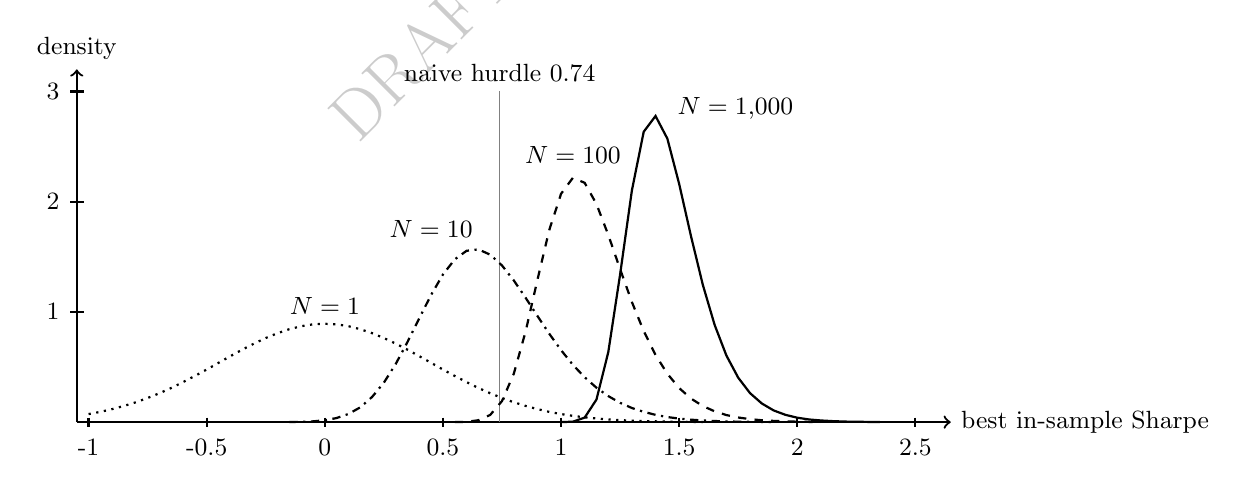
\begin{tikzpicture}[x=3cm,y=1.4cm,thick]
        \draw[->] (-1.05,0) -- (2.65,0) node[right,font=\small] {best in-sample Sharpe};
        \draw[->] (-1.05,0) -- (-1.05,3.2) node[above,font=\small] {density};
        \foreach \x in {-1,-0.5,0,0.5,1,1.5,2,2.5} {
            \draw (\x,0.04) -- (\x,-0.04);
            \node[below,font=\small] at (\x,-0.06) {\x};
        }
        \foreach \y in {1,2,3} {
            \draw (-1.02,\y) -- (-1.08,\y);
            \node[left,font=\small] at (-1.08,\y) {\y};
        }
        \draw[thin,gray] (0.74,0) -- (0.74,3.0) node[above,font=\small,text=black] {naive hurdle $0.74$};
        \draw[dotted] plot coordinates {(-1.00,0.073) (-0.95,0.093) (-0.90,0.118) (-0.85,0.147) (-0.80,0.180) (-0.75,0.219) (-0.70,0.262) (-0.65,0.310) (-0.60,0.363) (-0.55,0.419) (-0.50,0.477) (-0.45,0.538) (-0.40,0.598) (-0.35,0.657) (-0.30,0.712) (-0.25,0.763) (-0.20,0.807) (-0.15,0.843) (-0.10,0.870) (-0.05,0.887) (0.00,0.892) (0.05,0.887) (0.10,0.870) (0.15,0.843) (0.20,0.807) (0.25,0.763) (0.30,0.712) (0.35,0.657) (0.40,0.598) (0.45,0.538) (0.50,0.477) (0.55,0.419) (0.60,0.363) (0.65,0.310) (0.70,0.262) (0.75,0.219) (0.80,0.180) (0.85,0.147) (0.90,0.118) (0.95,0.093) (1.00,0.073) (1.05,0.057) (1.10,0.043) (1.15,0.033) (1.20,0.024) (1.25,0.018) (1.30,0.013) (1.35,0.009) (1.40,0.007) (1.45,0.005) (1.50,0.003) (1.55,0.002) (1.60,0.001)};
        \draw[dash dot] plot coordinates {(-0.15,0.001) (-0.10,0.003) (-0.05,0.007) (0.00,0.017) (0.05,0.037) (0.10,0.074) (0.15,0.134) (0.20,0.228) (0.25,0.358) (0.30,0.527) (0.35,0.727) (0.40,0.943) (0.45,1.154) (0.50,1.339) (0.55,1.476) (0.60,1.554) (0.65,1.567) (0.70,1.519) (0.75,1.421) (0.80,1.285) (0.85,1.128) (0.90,0.963) (0.95,0.802) (1.00,0.653) (1.05,0.520) (1.10,0.407) (1.15,0.312) (1.20,0.236) (1.25,0.175) (1.30,0.128) (1.35,0.093) (1.40,0.066) (1.45,0.046) (1.50,0.032) (1.55,0.022) (1.60,0.015) (1.65,0.010) (1.70,0.006) (1.75,0.004) (1.80,0.003) (1.85,0.002) (1.90,0.001)};
        \draw[dashed] plot coordinates {(0.55,0.000) (0.60,0.003) (0.65,0.017) (0.70,0.065) (0.75,0.191) (0.80,0.439) (0.85,0.822) (0.90,1.290) (0.95,1.742) (1.00,2.071) (1.05,2.216) (1.10,2.171) (1.15,1.978) (1.20,1.698) (1.25,1.388) (1.30,1.089) (1.35,0.826) (1.40,0.609) (1.45,0.439) (1.50,0.309) (1.55,0.214) (1.60,0.146) (1.65,0.098) (1.70,0.064) (1.75,0.042) (1.80,0.027) (1.85,0.017) (1.90,0.011) (1.95,0.007) (2.00,0.004) (2.05,0.002) (2.10,0.001)};
        \draw[solid] plot coordinates {(1.00,0.000) (1.05,0.004) (1.10,0.041) (1.15,0.205) (1.20,0.635) (1.25,1.339) (1.30,2.103) (1.35,2.634) (1.40,2.777) (1.45,2.572) (1.50,2.161) (1.55,1.688) (1.60,1.247) (1.65,0.883) (1.70,0.604) (1.75,0.403) (1.80,0.263) (1.85,0.169) (1.90,0.106) (1.95,0.066) (2.00,0.040) (2.05,0.024) (2.10,0.015) (2.15,0.009) (2.20,0.005) (2.25,0.003) (2.30,0.002) (2.35,0.001)};
        \node[font=\small] at (0.0,1.05) {$N=1$};
        \node[font=\small] at (0.45,1.75) {$N=10$};
        \node[font=\small] at (1.05,2.42) {$N=100$};
        \node[font=\small,right] at (1.45,2.85) {$N=1{,}000$};
    \end{tikzpicture}
\end{bookfigure}

The table reports averages; Figure~\ref{fig:best_of_n_density} shows the whole distribution behind them. Each added order of magnitude in $N$ moves the density of the winning Sharpe ratio to the right and makes it narrower: the most likely best-of-ten figure is $0.64$, the most likely best-of-a-thousand $1.39$. The naive hurdle of $0.74$ is cleared by luck alone with probability $5\%$ when one strategy is tested, $40.1\%$ when ten are, and $99.4\%$ when a hundred are, so for a search of that size clearing it says almost nothing.


Take $N = 100$: five short windows, five long windows, and four exit rules, a search most researchers would call modest. The expected best in-sample annualized Sharpe ratio is $1.12$ though every one of the hundred is worthless by construction, and a Monte Carlo of ten thousand such searches averages $1.118$ against the analytic $1.121$. That clears the naive $0.74$ hurdle comfortably and would usually be presented as a strong result, whereas the honest hurdle for the best of a hundred is $1.47$, almost twice. Out of sample the question is settled: the winner earns a mean Sharpe ratio of $+0.004$, loses money outright $49.6\%$ of the time, and the in-sample to out-of-sample rank correlation across the hundred is $+0.001$. The winner of a search is not better than what it beat. It is luckier, and luck does not persist into the next sample.

Three responses follow, and none of them is to stop searching. Report $N$, since a backtest presented without the number of configurations tried cannot be evaluated. Compare the reported figure against the best-of-$N$ hurdle rather than zero, as the deflated Sharpe ratio\index{deflated Sharpe ratio}\index{Sharpe ratio!deflated} of Bailey and L\'opez de Prado does, discounting a figure by how much a search of that size would inflate it and adjusting for the non-normality of real returns. And recognize that neighboring grid points are highly correlated (a 49-day and a 50-day moving average produce nearly identical positions), so the number of \emph{independent} trials sits well below the raw count: correlating every pair at $0.5$ lowers the mean best Sharpe ratio to $0.80$, what about eighteen independent trials would give rather than a hundred.

What none of it can manufacture is data: for a strategy whose \emph{true} annualized Sharpe ratio is $0.5$, a respectable edge, separating it from zero in a single pre-specified test takes about eleven years of daily returns, and clearing a hundred-configuration search about forty-three. Little strategy research runs on anything near that history, the strongest argument for pre-specifying a few economically motivated candidates, as Section~\ref{sec:taxonomy} framed them, rather than letting a grid search decide what the hypothesis should have been.

\subsection{Implementation Shortfall and Transaction Cost Analysis}\index{implementation shortfall}\index{transaction cost analysis (TCA)}\index{execution algorithms!implementation shortfall}

The gap between a strategy's theoretical performance, computed from the prices a signal was based on, and its realized performance, computed from the prices at which trades were executed, is called implementation shortfall, $\text{Execution Price} - \text{Decision Price}$. For the TWAP execution in Section~\ref{sec:twap-vwap}, if the decision to buy was made at \$50.00 (the decision price) but the order was executed via TWAP at \$50.07, the implementation shortfall is $\$50.07 - \$50.00 = \$0.07$ per share, $14$ basis points, or \$70 on the 1,000-share order. This number bundles every friction in this chapter: the market impact of Section~\ref{sec:market-impact}, the timing risk of Section~\ref{sec:optimal-execution}, and any price drift between decision and execution unrelated to the trade. It is the standard metric of transaction cost analysis (TCA) for judging whether a desk's execution adds or subtracts value relative to the decisions it implements. A strategy profitable on decision prices can prove unprofitable once realistic shortfall is subtracted, which is why serious backtesting should model transaction costs explicitly\index{transaction costs!execution} rather than assume execution at the prices a signal was computed from.

\section{Machine Learning and Event-Driven Signals}

Every signal so far, the moving-average crossover and the pairs-trading $z$-score, is a simple, interpretable rule with a handful of parameters. The classification and regression methods of Chapter~\chnum{ml} can generate richer ones: a gradient-boosted tree or neural network trained on many engineered features (lagged returns, rolling volatilities, volume features) can capture nonlinear patterns a fixed-form rule cannot represent. This part develops the features such a model is given and the discipline that keeps a flexible model honest, then turns to signals that arrive as events rather than continuous series.

\subsection{A Head-to-Head Test: Gradient Boosting versus Logistic Regression on a Regime Interaction}
\label{sec:ml-trading-signal}\index{gradient boosting!regime interaction}

The twelve-day price series of the feature-engineering catalog below is far too short to fit any model, so testing the claim above requires a longer history. The companion notebook builds 5,000 days of returns with volatility clustering\index{volatility clustering}, using the GARCH-style recursion of Chapter~\chnum{timeseries}, and layers a regime interaction on top: three-day momentum continues in calm, low-volatility stretches but reverses in turbulent ones. A logistic regression's additive coefficients cannot represent this, since one coefficient on momentum cannot be positive in one regime and negative in another. A logistic regression and a gradient-boosted classifier are trained on the same three features from Table~\ref{tab:trading_features}, on the first 3,500 simulated days, and evaluated on the final 1,496, following the walk-forward discipline, since time-ordered data cannot be split randomly without leaking future information.

Logistic regression reaches a held-out AUC of\index{area under the curve (AUC)}\index{gradient boosting!versus logistic regression} $0.5130$, barely above a coin flip's $0.50$, because its additive structure cannot capture a momentum effect that flips sign with the regime. Gradient boosting reaches $0.5328$, a modest improvement that holds up across random seeds, with feature importances of $0.423$ (momentum), $0.388$ (volatility), and $0.189$ (RSI) showing it draws on momentum and volatility jointly. Both AUCs are deliberately modest: financial returns have a low signal-to-noise ratio, as Chapter~\chnum{ml} cautioned, so an AUC in the low $0.50$s is a realistic stand-in for a real signal's small edge. Gradient boosting captures an interaction a linear-in-its-features model structurally cannot, even though the edge, like most real ones, is small.

\subsection{A Feature-Engineering Catalog for Trading Signals}
\label{sec:trading-feature-engineering}\index{feature engineering!trading signals}\index{trading signal!feature catalog}

Chapter~\chnum{ml} developed the general feature patterns (ratios, lagged and rolling windows, interaction terms, categorical encodings) used across this book's applications. Trading signals draw on a narrower catalog built almost entirely from price, volume, and order-book history, in four families. \textbf{Price-based} features summarize recent direction and magnitude: momentum, the trailing return over a fixed lookback window, and realized volatility, the rolling standard deviation of returns over the same window\index{realized volatility}, with the moving averages of Section~\ref{sec:ma-crossover} a third. \textbf{Technical indicators} repackage price history\index{technical indicators} into a bounded, more interpretable scale: the Relative Strength Index (RSI)\index{Relative Strength Index (RSI)}, the Absolute Price Oscillator (APO)\index{Absolute Price Oscillator (APO)}, the difference between a fast and a slow exponential moving average, and Bollinger Bands\index{Bollinger bands}, which wrap a moving average in a pair of volatility-scaled upper and lower bands, all three worked through numerically below.

\textbf{Volume-based} features, raw volume, dollar volume (price times volume), and volume relative to its own recent average, capture how much conviction accompanies a price move, which no price-based feature can see. \textbf{Microstructure-based} features draw on Chapter~\chnum{markets} and this chapter: the bid-ask spread and the order-flow imbalance behind Kyle's model\index{order flow imbalance (OFI)} in Section~\ref{sec:kyle-model} change on the timescale of individual trades rather than daily closes and carry information a price-based feature never sees.

\subsection{Momentum, Realized Volatility, and RSI}
\label{sec:momentum-rsi}\index{technical indicators!RSI}

Table~\ref{tab:trading_features} computes three of these features from the twelve-day price series of Section~\ref{sec:ma-crossover}: a 3-day momentum ($\text{Mom3}_t = P_t/P_{t-3} - 1$), a 3-day realized volatility (the rolling standard deviation of the three most recent daily returns), and a 3-period RSI, $\text{RSI} = 100 - 100/(1+RS)$ where $RS$ is the average of the window's positive price changes (gains) divided by the average magnitude of its negative changes (losses).

\begin{booktable}[htbp]{Three engineered trading-signal features, computed from Section~\ref{sec:ma-crossover}'s twelve-day price series}{tab:trading_features}
\begin{tabular}{lrrrr}
\toprule
Day & Price & Mom3 (\%) & Vol3 (\%) & RSI3 \\
\midrule
4  & 106 & 6.00   & 0.781 & 100.00 \\
5  & 110 & 8.91   & 0.732 & 100.00 \\
6  & 115 & 11.65  & 0.667 & 100.00 \\
7  & 119 & 12.26  & 0.450 & 100.00 \\
8  & 118 & 7.27   & 2.328 & 90.00 \\
9  & 114 & $-0.87$  & 2.835 & 44.44 \\
10 & 109 & $-8.40$  & 1.493 & 0.00 \\
11 & 104 & $-11.86$ & 0.523 & 0.00 \\
12 & 100 & $-12.28$ & 0.313 & 0.00 \\
\bottomrule
\end{tabular}
\end{booktable}

The three columns tell complementary stories about the same twelve days. Momentum tracks the trend, rising through day 7 and falling steadily thereafter, mirroring the price series.

Realized volatility does something momentum cannot. It stays low throughout the smooth days-4-through-7 uptrend ($0.45\%$ to $0.78\%$) and then spikes, to $2.3\%$ and $2.8\%$, at the days 8 and 9 reversal that Section~\ref{sec:ma-crossover} identified as the crossover strategy's whipsaw. That is an instance of the volatility clustering\index{volatility clustering} of Chapter~\chnum{timeseries}'s GARCH material: volatility rises around regime changes, not uniformly through time, which is why realized volatility is a useful predictive feature and not merely a risk-management input.

RSI shows a limitation alongside its usefulness. Because every change in the days-4-through-7 window is positive, RSI saturates at $100$ for four consecutive days, the conventional ``overbought'' signal, but cannot distinguish a mild uptrend from an explosive one once every recent change has the same sign; it falls as quickly to a saturated $0$ (``oversold'') once every recent change turns negative. A model trained only on RSI could not tell days 4 through 7 apart, despite their different momentum. Practitioners therefore feed a model both a bounded indicator like RSI and the underlying continuous features, such as momentum and realized volatility, letting the model learn how much weight each deserves rather than discarding what a saturated indicator throws away.

\subsection{Two Further Technical Indicators}
\label{sec:technical-indicators}\index{technical indicators!APO}\index{technical indicators!Bollinger bands}

Two further indicators are common enough to work through alongside RSI, both computed from an exponentially weighted moving average (EMA)\index{moving average!exponential} rather than the simple moving average of Section~\ref{sec:ma-crossover}: an EMA weights recent prices more heavily, updating as $\text{EMA}_t = \lambda P_t + (1-\lambda)\text{EMA}_{t-1}$ with smoothing factor $\lambda = 2/(N+1)$ for an $N$-period window, seeded at the first available price.

The \textbf{Absolute Price Oscillator (APO)} is the difference between a fast and a slow EMA, $\text{APO}_t = \text{EMA}^{\text{fast}}_t - \text{EMA}^{\text{slow}}_t$. Industry practice typically uses a 10-day fast and 40-day slow window (or, in the related MACD indicator, a 12-day and 26-day pair smoothed by a signal line), but Table~\ref{tab:indicators}, which also carries the Bollinger Bands introduced next, uses a 3-day and 6-day pair, scaled down to the twelve-day series as Section~\ref{sec:ma-crossover} scaled its moving-average windows.

\begin{booktable}[htbp]{Two further technical indicators on the same twelve-day price series: the Absolute Price Oscillator (3-day and 6-day EMA) and Bollinger Bands (5-day SMA, $k=2$)}{tab:indicators}
\begin{tabular}{lrrrrrrr}
\toprule
Day & Price & EMA3 & EMA6 & APO & SMA5 & Upper & Lower \\
\midrule
1  & 100 & 100.000 & 100.000 & 0.000 & 100.000 & 100.000 & 100.000 \\
2  & 101 & 100.500 & 100.286 & 0.214 & 100.500 & 101.500 & 99.500 \\
3  & 103 & 101.750 & 101.061 & 0.689 & 101.333 & 103.828 & 98.839 \\
4  & 106 & 103.875 & 102.472 & 1.403 & 102.500 & 107.083 & 97.917 \\
5  & 110 & 106.938 & 104.623 & 2.314 & 104.000 & 111.266 & 96.734 \\
6  & 115 & 110.969 & 107.588 & 3.381 & 107.000 & 117.040 & 96.960 \\
7  & 119 & 114.984 & 110.849 & 4.136 & 110.600 & 122.234 & 98.966 \\
8  & 118 & 116.492 & 112.892 & 3.600 & 113.600 & 123.447 & 103.753 \\
9  & 114 & 115.246 & 113.208 & 2.038 & 115.200 & 121.575 & 108.825 \\
10 & 109 & 112.123 & 112.006 & 0.117 & 115.000 & 122.043 & 107.957 \\
11 & 104 & 108.062 & 109.719 & $-1.657$ & 112.800 & 124.071 & 101.529 \\
12 & 100 & 104.031 & 106.942 & $-2.911$ & 109.000 & 122.023 & 95.977 \\
\bottomrule
\end{tabular}
\end{booktable}

The APO column tells the same trend story as momentum through an EMA's smoother lens: it is positive and climbing throughout the days-1-through-7 uptrend, peaking at $4.136$ at day 7's local high, then falls and turns negative by day 11 once the fast EMA crosses below the slow one, a lagging but interpretable confirmation of the reversal the crossover strategy was built to detect.

\textbf{Bollinger Bands} wrap a simple moving average in bands a fixed number of standard deviations above and below it: $\text{Middle}_t = \text{SMA}_t$, $\text{Upper}_t = \text{SMA}_t + k\cdot\sigma_t$, and $\text{Lower}_t = \text{SMA}_t - k\cdot\sigma_t$, where $\sigma_t$ is the rolling standard deviation of price (not return) over the same window as the moving average and $k$ is conventionally set to $2$. Industry practice typically uses a 20-day window; the table instead uses a 5-day window, for the same reason it shortened the EMA windows above.

The band width (upper minus lower) is itself a volatility indicator, telling the same story as Table~\ref{tab:trading_features}'s Vol3 column: the bands are tight while days 1 through 5 climb smoothly, then widen sharply from day 6 and stay wide through day 12, tracking the days-8-and-9 spike Vol3 flagged and the GARCH-style clustering of Chapter~\chnum{timeseries}, expressed geometrically around the price chart. Both indicators transform the rolling mean and dispersion already summarized by momentum and realized volatility, so neither supplies information a model could not in principle extract from those two. Their value is the packaging: a chart a human trader can read at a glance, which is why both remain popular in practitioner tools even though a machine-learning pipeline can work from the underlying features.

\subsection{Putting the Features to Work}
\label{sec:features-to-work}

Computing indicators is only the first step. The four topics below cover what surrounds them in a working strategy: a market-wide regime filter, two data disciplines, the move from features to a portfolio, and out-of-sample validation.

\subsubsection*{A Market-Wide Feature: The VIX}

Every indicator so far is computed from a single asset's price history and looks backward. The CBOE Volatility Index (VIX)\index{CBOE Volatility Index (VIX)}, introduced in Chapter~\chnum{valuation} as the market-implied volatility aggregated across S\&P 500 index options, is a different kind of feature\index{CBOE Volatility Index (VIX)!as a trading feature}: a market-wide, forward-looking measure of expected volatility over the next 30 days.

Strategies routinely use the VIX level, or its rate of change, as a regime filter\index{regime filter} on top of asset-specific signals. A momentum strategy's whipsaw risk, of which Section~\ref{sec:ma-crossover}'s days-8-and-9 reversal is a small-scale illustration, tends to be worse when VIX is elevated and the market unsettled. A strategy might therefore reduce position sizes, widen its stop-losses, or stand aside once VIX crosses a threshold, rather than treating every day as statistically identical. Because VIX is tradable, through futures, options, and exchange-traded products, some strategies also trade VIX-linked instruments as a hedge against the market volatility that erodes asset-specific strategies' returns.

\subsubsection*{Two Disciplines: Point-in-Time Data and Stationarity}\index{point-in-time data}\index{stationarity!for trading features}

Two disciplines from earlier chapters apply to every feature in Table~\ref{tab:trading_features}. First, the point-in-time rule Section~\ref{sec:ma-crossover} enforced applies to every engineered feature: a momentum, volatility, or RSI value computed from prices through day $t$ can only trade day $t+1$'s return, never day $t$'s. A backtest that lines up a feature with the same day's return it was partly computed from commits the data leakage Chapter~\chnum{ml} warned against, only harder to spot because the feature looks like an input rather than an answer.

Second, Chapter~\chnum{timeseries}'s stationarity material explains why every feature in the table is a \emph{transformation} of price rather than the raw price level. A price can trend arbitrarily far from its starting value over a dataset (the non-stationarity of the unit-root discussion), so a model trained on raw price levels from one period would have to extrapolate to price ranges it never saw. Momentum, RSI, and volume ratios are normalized to a roughly stationary, comparable scale regardless of price level or period, which is why they, rather than price, are handed to a model.

\subsubsection*{From Features to Portfolio Construction}

A quantitative equity manager typically does not predict an absolute return but trains a model to produce a cross-sectional ranking of a universe of stocks from most to least attractive over the next period, since a ranking is often easier to learn reliably and more useful for portfolio construction than a point forecast of each return. The ranking feeds into the mean-variance and risk-parity machinery of Chapter~\chnum{portfolio}: the optimizer takes the model's scores as its expected-return input, combining a machine-learning forecast with classical risk-management discipline, the layered, classical-plus-modern pipeline emphasized throughout this book.

Beyond price and volume history, increasingly important feature sources are order-book microstructure data, such as the order-flow imbalance (the net difference between resting buy and sell volume at the top of the book) behind Kyle's model in Section~\ref{sec:kyle-model}, and the alternative data of Chapter~\chnum{altdata}\index{alternative data}, such as satellite imagery, web traffic, or transaction data, which can supply predictive information independent of the price and volume history every other participant observes.

\subsubsection*{Overfitting and Walk-Forward Validation}\index{overfitting!in backtests}

The overfitting\index{overfitting} concern of Section~\ref{sec:backtest-overfit} applies with particular force here, for an additional reason: a flexible model does not merely search a grid of parameters but an enormous implicit space of functional forms, so its effective $N$ is larger than any explicit configuration count and harder to deflate for. Walk-forward validation, introduced in Chapter~\chnum{timeseries}\index{walk-forward validation}\index{cross-validation!walk-forward} because a random train-test split leaks future information in time-ordered data, is essential for any machine-learning trading signal. Even a walk-forward-validated signal must still be evaluated net of implementation shortfall and market impact before its statistical performance counts as a tradable economic edge.

\subsubsection*{Is This Signal Causal?}\index{causal inference}

A signal that survives walk-forward validation has earned the right to be called predictive, not causal; Chapter~\chnum{ml}'s section on prediction versus causation (Section~\chnum{ml}.3.6) explains the difference. For pure trading it often does not matter: a feature that reliably precedes returns is worth trading whether it moves prices or merely shares a cause with whatever does. It matters the moment the strategy's own behavior, or the market's, changes the relationship. A momentum signal may work because slow-moving capital chases recent winners; if a regime filter, a change in index rules, or other funds trading the same feature alter that flow, the correlation the model learned can vanish without any warning visible in its historical fit. The questions Chapter~\chnum{ml} asks of a credit-limit decision apply here too. What mechanism would make the feature move prices? Is there a confounder, such as market-wide volatility, that drives both the feature and the return? Would the relationship survive an intervention, such as the strategy itself trading at scale? A signal backed by a plausible mechanism, and still present after the obvious confounders are controlled for, is more likely to persist out of sample than one discovered only because it fit.

These methods apply across a wide range of horizons, from a multi-day pairs trade to an execution algorithm working an order over an afternoon. At the shortest end, high-frequency trading pushes this chapter's ideas\index{high-frequency trading (HFT)} (order types, market impact, inventory management) down to milliseconds or microseconds, where the physical latency of transmitting information and orders becomes a first-order concern. With its own technology, market-making techniques, and regulatory debates, high-frequency trading receives its own treatment in Chapter~\chnum{hft}.

\subsection{News and Event-Driven Trading}\index{news and event-driven trading}

A distinct signal category trades on the arrival of new information: an earnings announcement, a central bank rate decision, a merger announcement, or a news headline. Because the content of such events is largely unpredictable (a firm's earnings-release date is known in advance, but not what it will say), event-driven strategies focus less on predicting when a signal will arrive and more on reacting to it faster and more accurately than other participants.

This is where the natural language processing methods of Chapter~\chnum{nlp} meet this chapter's execution machinery. Extracting a sentiment score or structured summary from an earnings call transcript\index{sentiment analysis!trading signal}\index{earnings call} or news wire is only half of an event-driven strategy. The other half is converting that signal into a position quickly enough to matter (a slowly generated signal may arrive after the price has already moved) and executing the trade while managing the market impact and implementation shortfall of Sections~\ref{sec:market-impact} and~\ref{sec:optimal-execution}. Those costs are often most severe right after a major news event, when liquidity is thin and many participants are trading on the same information at once.

\section{Market Structure and Safeguards}

Automated trading interacts with other automated trading, sometimes in ways nobody designed. This part covers the safeguards the market imposes on that interaction, and one episode in which a firm's own missing safeguards destroyed it in forty-five minutes.

\subsection{Circuit Breakers and Trading Halts}\index{circuit breaker!trading halts}

Chapter~\chnum{markets} described the 2010 Flash Crash\index{Flash Crash of 2010}, in which the Dow Jones Industrial Average fell and then recovered nearly 1,000 points within minutes, driven in significant part by algorithmic systems interacting in ways no participant had designed or anticipated. One regulatory response to that episode, and to the risk that automated trading can amplify a price move far beyond what fundamentals justify, is the circuit breaker\index{circuit breaker}: an automatic, exchange-wide (or single-stock) trading halt triggered once price moves beyond a threshold within a time window. It gives participants, human and algorithmic, a pause to assess whether a move reflects new information or a mechanical, self-reinforcing feedback loop like the Flash Crash.

Circuit breakers interact with the execution and market-making concepts of this chapter. A market maker running the Avellaneda-Stoikov framework of Section~\ref{sec:inventory} must decide how to handle a position when trading is suddenly halted, since the model assumes it can trade continuously, an assumption a halt violates by design. Similarly, a TWAP or VWAP schedule spread across a day needs explicit logic for a halt partway through, either pausing and resuming or reassessing the remaining plan, since proceeding as though nothing happened could execute the remaining slices at prices that no longer reflect the conditions the schedule was designed for.

\vignetteheading{\subsection}{knight}{The Knight Capital Trading Glitch}\index{Knight Capital trading glitch}

On August 1, 2012, Knight Capital Group, then one of the largest market makers in US equities, deployed new trading software to its production servers. A deployment error left obsolete code active on one of eight servers; combined with the new software, it caused the firm's systems to send a rapid, unintended stream of erroneous orders into the market. Within approximately 45 minutes, before the problem was identified and the system halted, Knight had accumulated large, unintended positions across dozens of stocks. Unwinding them cost about \$440 million, more than its capital cushion could absorb; its share price fell by roughly three-quarters within two days, and the loss forced an emergency capital infusion and ultimately a rescue merger with a competitor.

The episode illustrates the technology and latency risk flagged in this chapter's challenges section, and the failure was not a flawed trading strategy. Knight's algorithms were not making a bad prediction or a poorly calibrated\index{calibration} risk-reward trade-off; a deployment error caused the firm's execution infrastructure, the machinery this chapter has treated as neutral plumbing, to behave in a way no human intended or approved.

The speed that makes algorithmic and high-frequency trading profitable is what turned a deployment bug into a \$440 million loss in well under an hour: a human-paced operation making the same error would likely have intervened long before losses reached that scale. The lesson generalizes to the model risk management\index{model risk management} framework of Chapter~\chnum{marketrisk}: an algorithmic trading system requires the same independent testing, staged deployment, real-time monitoring, and kill-switch capability\index{kill switch} as a bank's VaR\index{Value at Risk (VaR)} or credit model, because the speed that makes automation valuable makes an undetected error catastrophic.

\section{Challenges in Algorithmic Trading and Market Microstructure}

Several challenges recur across nearly every algorithmic trading application.

\textbf{Backtest overfitting.}\index{backtest overfitting} With enough data and candidate strategies, some rule will appear profitable by chance, the multiple-testing concern raised in Chapters~\chnum{ml},~\chnum{timeseries}, and~\chnum{portfolio}. Section~\ref{sec:backtest-overfit} put a number on it: searching a hundred worthless configurations yields an expected best in-sample Sharpe ratio of $1.12$, and the winner has no out-of-sample edge. A strategy found by searching many parameter combinations must be validated out of sample, and deflated for the size of the search, far more skeptically than one derived from a pre-specified economic hypothesis.

\textbf{Market impact is itself uncertain and strategy-dependent.}\index{market impact} The clean numbers in Section~\ref{sec:market-impact} come from a simplified, static order book; real impact depends on volatility, on whether others can detect and react to a large order being worked, and on liquidity conditions that vary over time, making it harder to estimate than a strategy's other inputs.

\textbf{Latency and technology risk.}\index{latency} Execution and market-making strategies depend on fast, reliable technology, and a software bug, a connectivity failure, or delayed market data can turn a sound strategy into a source of real, sometimes rapid, losses: the operational risk of Chapter~\chnum{oprisk} in a domain where a failure compounds within seconds rather than days.

\textbf{Adverse selection from faster participants.}\index{adverse selection!in market making} A posted limit order risks being filled by a faster or better-informed participant when that is disadvantageous, the adverse-selection component of the bid-ask spread introduced in Chapter~\chnum{markets}; the more of this risk a strategy bears, the wider the effective spread it must earn to break even.

\textbf{Regulatory and market-structure change.} Algorithmic and high-frequency trading operate within an evolving regulatory framework (Regulation NMS and its analogues\index{Regulation NMS (Reg NMS)}), and a strategy whose profitability depends on a specific market-structure feature, such as an exchange's fee structure or order-matching rule, can see that edge disappear or reverse if the rules change.

\textbf{Crowding in statistical arbitrage.}\index{statistical arbitrage} The 2007 quant quake of Section~\ref{sec:stat-arb} is a documented instance of a general hazard. When many firms independently discover and trade similar statistical relationships, their positions become correlated in a way none can observe from its own book. A shock or forced unwind at one large fund can then trigger simultaneous, self-reinforcing losses across ostensibly unrelated strategies, the crowding risk Chapter~\chnum{portfolio} raised for long-horizon factor investing, unfolding over hours rather than months.

\textbf{Exchange fee structures and rebates.} Many exchanges charge a fee to remove liquidity (executing against a resting order) and pay a rebate to add it (posting a resting limit order that another participant later executes against). This maker-taker pricing model\index{maker-taker pricing model} creates incentives independent of the trading signal. Profitability can depend materially on whether a strategy posts passive limit orders or crosses the spread, and two strategies with identical signals can have different net profitability purely because of how each interacts with an exchange's fee schedule. A realistic backtest, following the transaction-cost discipline of Section~\ref{sec:backtest-metrics}, should account for fees and rebates explicitly, since a few basis points of fee difference, compounded across thousands of trades, can separate a strategy that is profitable after costs from one that only appears to be. The fee schedule is one more component of implementation shortfall, no less real for being easy to overlook.

\textbf{Capacity constraints on strategy scale.} A strategy backtested at a small notional size can look highly attractive on a risk-adjusted basis. But the market impact costs of Section~\ref{sec:market-impact} grow faster than linearly with order size, as $Q^{3/2}$ in total dollars under the square-root law of Section~\ref{sec:square-root-impact}. The same strategy at ten or a hundred times the capital can see its net returns deteriorate sharply, or turn negative, well before it exhausts its statistical edge; that section's example supports at most \$61.4 million profitably. Capacity is an economic limit on how much capital any trading idea, however sound, can absorb.

\notocsection{Key Takeaways}

Converting a trading signal into a position, and a position into a profit-and-loss series, means confronting the microstructure realities of Chapter~\chnum{markets}: the bid-ask spread, the limited depth at each price level, and the price impact of consuming that depth too quickly. The Kyle model interprets price impact as compensation for trading against better-informed counterparties; TWAP and VWAP are standard execution benchmarks; and the Almgren-Chriss framework formalizes the trade-off between market impact and timing risk.

Market making becomes an explicit inventory-management problem, and pairs trading becomes a complete, backtestable strategy once entry and exit rules are applied out of sample, a logic that extends to statistical arbitrage across many assets using the factor models of Chapter~\chnum{portfolio}. The execution and market-making models are closed-form answers bought with strong assumptions, and Chapter~\chnum{rl} revisits each as a sequential decision problem solved by learning rather than algebra.

Evaluating a strategy requires more than a return figure: the Sharpe ratio, maximum drawdown, and hit rate each reveal a different dimension of performance, and each must be computed net of realistic transaction costs and implementation shortfall, since the gap between theoretical and realized performance often separates a strategy that looks good on paper from one worth trading.

The Knight Capital vignette and the discussion of circuit breakers make a point that recurs throughout this book: the technology and market structure around a trading decision are not neutral plumbing but sources of risk in their own right, deserving the governance discipline Chapter~\chnum{marketrisk} developed for risk models.

A statistically sound backtest is necessary but never sufficient. Fees, capacity limits, crowding, and the risk of a software or operational failure all sit between a promising historical result and a profitable, sustainable trading operation. The machine learning signals of Chapter~\chnum{ml} and the natural-language and alternative-data sources of Chapters~\chnum{nlp} and~\chnum{altdata} must clear the same hurdles before a sophisticated model becomes a trade that makes money net of these frictions.

The next chapter narrows the focus to the millisecond-scale end of this spectrum, where every idea introduced here still applies but is compressed into a timescale where speed itself becomes a primary competitive advantage.

\notocsection{Suggested Exercises}

\begin{enumerate}[exercises]
    \item Using Table~\ref{tab:ma_crossover}, verify by hand that the 3-day and 6-day moving averages at day 8 are 117.33 and 111.83, and explain why the strategy signal remains long (1) at that point.
    \item Recompute the moving-average crossover strategy's cumulative return using a 2-day short average and a 4-day long average on the same twelve-day price series, and compare the resulting signal timing to the 3-day/6-day version in the text.
    \item A 500-share market order walks through an order book with 200 shares available at \$30.00 and additional shares available at \$30.05. Compute the average execution price and the price impact in basis points relative to the best price.
    \item Using Table~\ref{tab:twap_vwap}, compute the TWAP and VWAP execution prices for a 2,000-share order, and explain why they differ.
    \item Explain, in your own words, why an inventory-skewing market maker (Section~\ref{sec:inventory}) adjusts both its bid and ask when it accumulates a large position, rather than adjusting only the side of the quote nearest the current inventory.
    \item Using the extended pairs-trading data in Table~\ref{tab:pairs_backtest}, compute the trade's profit and loss if the position were instead closed at day 9 rather than day 10, and compare it to the day-10 exit computed in the text.
    \item A strategy has a Sharpe ratio of $1.2$ and a maximum drawdown of $18\%$, while a second strategy has a Sharpe ratio of $0.8$ and a maximum drawdown of $5\%$. Discuss which strategy an investor with a low tolerance for large losses might prefer, and why Sharpe ratio alone would not reveal this consideration.
    \item A portfolio manager's decision price is \$100.00 and the resulting order is executed at an average price of \$100.12 on a 5,000-share order. Compute the implementation shortfall in basis points and in total dollars.
    \item Using Table~\ref{tab:trading_features}'s twelve-day price series, try to compute the 3-day momentum, 3-day realized volatility, and 3-period RSI at day 3, and explain why none of them is yet defined there under the chapter's definitions, while all three first become available at day 4.
    \item Explain, referencing Table~\ref{tab:trading_features}'s RSI column, why an indicator that saturates at $0$ or $100$ can lose information a model might otherwise use, and describe why feeding a model both RSI and the underlying momentum feature side by side addresses this limitation.
    \item Using Table~\ref{tab:indicators}, verify by hand that day 8's APO is $3.600$, and explain why APO does not turn negative until day 11, four days after day 7's price high, rather than exactly at it.
    \item Using Table~\ref{tab:indicators}, explain why the band width at day 7 (Upper minus Lower) is so much larger than at day 2, referencing this section's discussion of Table~\ref{tab:trading_features}'s Vol3 column.
    \item Explain why walk-forward validation, introduced in Chapter~\chnum{timeseries}, is essential when evaluating a machine-learning-based trading signal, and describe a specific way that a random train-test split could produce a misleadingly optimistic backtest.
    \item Pick two of the challenges listed in this chapter and describe a concrete scenario, not already used in the text, in which that challenge could cause an algorithmic trading strategy to lose money despite a statistically sound backtest.
    \item Using Table~\ref{tab:kyle_data}, verify by hand that Kyle's lambda is approximately 1.95 cents per thousand shares, and interpret what a much larger estimated lambda (say, 10 cents per thousand shares) would suggest about that market compared to the one in the text.
    \item Explain the difference between an iceberg order and trading in a dark pool, and describe one advantage and one disadvantage each has relative to posting a single, fully visible limit order.
    \item Describe how a market maker using the inventory-skewing logic of Section~\ref{sec:inventory} should adjust its behavior if trading in the underlying stock is suddenly halted by a circuit breaker, and explain what risk this halt introduces that continuous trading does not.
    \item Using the Avellaneda-Stoikov formulas in Section~\ref{sec:inventory}, recompute the reservation price, optimal spread, bid, and ask for a market maker with the same parameters as the worked example except that it is short $q=-8$ units instead of long 5, and explain why the resulting skew now points in the opposite direction.
    \item Explain why the Knight Capital case vignette is better understood as a technology and governance failure than as a bad trading strategy, and describe one specific model risk management practice from Chapter~\chnum{marketrisk} that, if followed, might plausibly have prevented or limited the loss.
    \item A statistical arbitrage fund holds 200 similar mean-reversion positions across a sector. Explain, referencing the 2007 quant quake, why this diversification might provide less protection than the number of positions alone would suggest.
    \item Using Table~\ref{tab:statarb}, explain why Stock W's large residual $z$-score alone does not tell a trader whether to put on the suggested trade, and describe what additional information (beyond the regression output) an analyst would want before shorting Stock W against its sector peers.
    \item A backtest of a value strategy is run only on stocks currently listed on a major exchange, using their full, publicly available price history. Identify the specific bias this introduces, referencing this chapter's discussion of backtesting pitfalls, and describe one concrete step a researcher could take to correct it.
    \item Using the Almgren-Chriss worked example, compute $\kappa$ and the resulting optimal trajectory $x_j$ for the same $250$-share order and $N=5$ intervals if risk aversion were $\phi=2$ instead of $0.5$ or $5$, and state whether the resulting schedule is more or less front-loaded than both trajectories computed in the text.
    \item Explain, in your own words, why the fully aggressive single-shot execution in the Almgren-Chriss worked example has zero timing-risk variance, and why this alone does not make it the risk-adjusted optimal strategy even for a highly risk-averse trader.
    \item \textbf{VWAP under a mistaken volume forecast.} Section~\ref{sec:twap-vwap} argues that a VWAP algorithm is only as good as its forecast of the day's volume curve. Using Table~\ref{tab:twap_vwap}'s prices and realized volumes, suppose an algorithm works a 1,000-share buy order according to a forecast volume profile of $15\%$, $20\%$, $25\%$, $15\%$, and $25\%$ across the five intervals. (a) Compute the realized-volume VWAP benchmark and the average price the algorithm actually achieves. (b) Report the shortfall against that benchmark in cents per share, in basis points, and in dollars on the full order. (c) Identify which intervals' forecast errors caused the shortfall and which one partially offset it, and explain why an error in an interval whose price sits close to the VWAP costs almost nothing.
    \item Using the square-root law and the capacity example of Section~\ref{sec:square-root-impact}, suppose the strategy's gross alpha per trade is $30$ rather than $50$ basis points, with everything else unchanged. (a) Compute the impact cost of a trade equal to $2\%$ of a stock's daily volume. (b) Find the assets under management at which net alpha falls to zero, and the size that maximizes dollar profit. (c) Explain why a $40\%$ cut in gross alpha shrinks the profit-maximizing fund size by much more than $40\%$.
    \item A stock trades at \$20 with an annual return volatility of $30\%$, and an execution desk splits each trading day into ten intervals. Convert this volatility into the units the Almgren-Chriss objective of Section~\ref{sec:optimal-execution} requires, and explain what would go wrong if $\sigma=0.30$ were entered into the formula directly.
    \item A researcher finds that stocks with a high order-flow imbalance at the close tend to rise the next morning, and the signal survives walk-forward validation. Following this chapter's discussion of whether a signal is causal, name one mechanism that would make the relationship causal, one confounder that could produce it without any causal link, and one change in market conditions under which you would expect it to stop working.
    \item \textbf{Challenge (real data).} Download at least two years of daily prices for a real, liquid stock (via \texttt{yfinance}) and implement this chapter's moving-average crossover strategy (Table~\ref{tab:ma_crossover}) using a 20-day short window and a 50-day long window. (a) Backtest the strategy's cumulative return against a simple buy-and-hold benchmark over the full sample, and compute both strategies' Sharpe ratios. (b) Using walk-forward validation (Chapter~\chnum{timeseries}) rather than a single in-sample backtest, split your sample into several sequential training/testing windows and report whether the strategy's out-of-sample Sharpe ratio holds up as well as its in-sample Sharpe ratio. (c) Compute the feature set in Table~\ref{tab:trading_features} (momentum, realized volatility, RSI) for your real price series, and discuss whether the volatility clustering the twelve-day example showed around its crossover reversal appears at your strategy's entry and exit points.
\end{enumerate}

\notocsection{Further Reading}

\begin{itemize}
    \item \frcite{almgren2001optimal} The original formalization of the market-impact-versus-timing-risk trade-off developed in Section~\ref{sec:optimal-execution}.
    \item \frcite{almgren2005direct} An estimation of permanent and temporary impact from a large set of institutional U.S. equity orders, the empirical counterpart of Section~\ref{sec:square-root-impact}'s square-root law.
    \item \frcite{toth2011anomalous} A theory of why metaorder impact grows with the square root of size, together with fresh empirical support for the law used in Section~\ref{sec:square-root-impact}.
    \item \frcite{appel2005technical} Written by the creator of the MACD indicator, the closely related, signal-line-smoothed cousin of the Absolute Price Oscillator used in Section~\ref{sec:technical-indicators}'s feature-engineering worked example.
    \item \frcite{avellaneda2008high} The original inventory-based market-making model summarized in Section~\ref{sec:inventory}.
    \item \frcite{bailey2014deflated} The source of the deflation adjustment recommended in Section~\ref{sec:backtest-overfit}, and the standard reference on backtest overfitting.
    \item \frcite{bollinger2001bollinger} Written by the creator of the Bollinger Bands indicator used in Section~\ref{sec:technical-indicators}'s feature-engineering worked example.
    \item \frcite{chan2013algorithmic} A practitioner-oriented treatment of strategy development and backtesting, including the pairs-trading and mean-reversion strategies extended in this chapter.
    \item \frcite{harris2003trading} A comprehensive treatment of order types, market structure, and execution that extends this chapter's introductory coverage and connects directly back to Chapter~\chnum{markets}.
    \item \frcite{kissell2013science} Covers transaction cost analysis and implementation shortfall, introduced in this chapter, in considerably greater quantitative depth.
    \item \frcite{kyle1985continuous} The original paper formalizing the price-impact model summarized in Section~\ref{sec:kyle-model}.
    \item \frcite{wilder1978new} The original source introducing the Relative Strength Index used in Section~\ref{sec:momentum-rsi}'s feature-engineering worked example.
    \item \frcite{gueant2013dealing} A rigorous, closed-form treatment extending the Avellaneda-Stoikov inventory model of Section~\ref{sec:inventory} to more realistic order-arrival assumptions.
    \item \frcite{patterson2012dark} A journalistic but well-researched account of the rise of dark pools, algorithmic trading, and the market-structure debates touched on in this chapter's discussion of order routing and venue choice.
\end{itemize}

\end{document}

